\section{Network Exposure}
\label{chap:proposal:exposure}

As outlined in Section \ref{sec:sba:nef}, the \acf{NEF} is the main \acs{5G} core network function responsible for exposing network capabilities to external (and possibly internal) consumers. To do so, it offers a set of standardized northbound \acsp{API} that mediate access between the \acs{5G} core and consuming \acsp{AF}, while abstracting internal network functions and their implementation details. In the proposed testbed, the \acs{NEF} also serves as the primary gateway to \acs{5G} network programmability. Nonetheless, CAMARA interfaces should be provided to offer the same capabilities at an higher level of abstraction.

The coexistence of both interfaces lets each vertical choose the abstraction level that best fits its needs. While the \acs{NEF} adheres to complex \acs{3GPP} specifications but offers greater flexibility and programmability, CAMARA provides simpler, developer-facing interfaces but providing less granular control over the network. Regardless of the abstraction level, exposing these interfaces to third parties requires a common governance mechanism through which verticals can access them in a controlled and secure manner. 

The \acs{3GPP} \acs{CAPIF} fulfills such role by providing under a single platform common procedures for the secure publication, discovery and consumption of capability exposure \acsp{API}. It supports \acsp{API} specified by \acs{3GPP} or by other industry consortia, making it applicable to the northbound \acsp{API} exposed by the \acs{NEF}, as well as those defined by CAMARA.

\subsection{\acs{NEF}}
\label{chap:proposal:exposure:nef}

In the context of the proposed testbed, three \acs{NEF} northbound \acsp{API} are considered to address distinct, yet complementary aspects of network application behavior. The \textit{AsSessionWithQoS} \acs{API} targets \acs{QoS} control, providing applications with the means to establish and manage application sessions with specific \acs{QoS} profiles designed to guarantee, for example, specific bandwidth or latency requirements~\cite{ETSI_TS_129_122_V18_8_0}. This supports use cases that depend on predictable network behavior, letting applications programmatically request connectivity with specific characteristics, such as guaranteed uplink throughput or traffic priority, without human intervention. Notable examples include \acs{PPDR} applications needing temporary network resources for sporadic emergencies, and real-time video applications requiring low latency (e.g. eHealth) or support for large audiences (e.g. live broadcasting).

However, passively relying on the \acs{QoS} session established via this \acs{API} is not sufficient, as undetected violations of network requirements directly risk the correct functioning of the Network Application. Therefore, there is a clear need for a mechanism capable of actively monitoring the network and detecting any violations of the defined \acs{QoS} in real time. The \textit{AnalyticsExposure} \acs{API} addresses this problem giving developers the ability to query network analytics and subscribe to analytics notifications~\cite{ETSI_TS_129_522_V18_11_0}, allowing applications to monitor network metrics and adapt their behavior according to the observed conditions.

\acs{QoS} violations and changes in network conditions are not the only criteria that can require adaptive application behavior. According to its use case, the network application may need to be notified about specific events in the \acs{3GPP} network, completely unrelated to \acs{QoS}, such as an \acs{UE} becoming unreachable or changing location. The \textit{MonitoringEvent} \acs{API} was designed to create and manage such monitoring event subscriptions~\cite{ETSI_TS_129_122_V18_8_0}, covering events such as location reporting, loss of connectivity, \acs{UE} reachability and roaming status.

These common events can trigger different operations depending on the vertical and application scenario. For example, a \acs{TL} platform may use location updates to trigger \acs{QoS} adjustments as a teleoperated vehicle enters geofenced zones~\cite{NextGenConnectivityDynamicQoS}. In this way, monitoring events complement the \textit{AsSessionWithQoS} \acs{API} by enabling applications to adapt their requested \acs{QoS} in response to changes in \acs{UE} state.

The testbed requires all three \acsp{API} to support the envisioned network application behavior. In the remainder of this section, a closer look is taken at the \textit{AsSessionWithQoS} and \textit{AnalyticsExposure} \acsp{API}, which will be addressed in the next chapter.

\subsubsection{AsSessionWithQoS \acs{API}}
\label{chap:proposal:exposure:nef:AsSessionWithQoS}

The \textit{AsSessionWithQoS} \acs{API}, originally defined in \acs{3GPP} TS~29.122~\cite{ETSI_TS_129_122_V18_8_0}, allows applications to configure sessions indicating the desired level of \acs{QoS} for a given traffic flow. Through notifications, the \acs{API} also informs the application whether the requested \acs{QoS} can be enforced in the network.

The interaction is initiated when the \acs{AS}/\acs{AF} (e.g. a network application) submits an HTTP POST request to the \acs{NEF}, carrying an \texttt{AsSessionWithQoSSubscription} resource body~\cite{ETSI_TS_129_122_V18_8_0}. This body comprises an extensive set of parameters whose presence is governed by conditional rules, depending on the remaining payload content and on the \acs{API} features supported by the \acs{5GC}. Rather than covering all of these parameters, this section focuses on the attributes that express the desired \acs{QoS} configuration.

These include the target \acs{UE}, typically identified by its \acs{IP} or \acs{MAC} address, although groups of \acsp{UE} (\texttt{extGroupId}) or a subscription identifier such as the \ac{GPSI} may also be used when the corresponding features are supported. The traffic flow subject to \acs{QoS} treatment is then described as an \acs{IP} flow (\texttt{flowInfo}) or an Ethernet flow (\texttt{ethFlowInfo}), in accordance with the type of address provided.

The requested \acs{QoS} for that flow can be defined through the \texttt{qosReference} attribute, which references pre-defined \acs{QoS} information (e.g. \acs{QCI}/\acs{5QI} and associated parameters defined by the operator), optionally complemented by \texttt{altQoSReferences}, an ordered list of alternative references ranked by priority. Alternatively, a list of alternative service requirements (\texttt{altQosReqs}) can also be specified, each containing an individual set of \acs{QoS} parameters, namely the guaranteed bandwidth in uplink (\texttt{gbrUl}) and downlink (\texttt{gbrDl}), the packet delay budget (\texttt{pdb}) and the packet error rate (\texttt{per}). Finally, the attribute \texttt{notificationDestination} supplies the \acs{URL} at which the application will receive all notification events.

The specification further defines attributes such as usage thresholds (\texttt{usageThreshold}), \acs{QoS} signalling control (\texttt{disUeNotif}), and requirements for time sensitive communications (\texttt{tscQosReq}), which are beyond the scope of the targeted used cases. It also supports \acs{QoS} monitoring, through which the application subscribes to the \texttt{QOS\_MONITORING} event to receive measurements on the established flow. These measurements are limited to packet delay (\texttt{qosMonInfo}), data rate (\texttt{qosMonDatRate}) and congestion information (\texttt{qosMonConReq}), which are usually not covered nor utilized in the examples found throughout the literature.

Following the creation request, the \acs{NEF} maps the supplied \acs{QoS} references/parameters and coordinates with the \acs{PCF} to enforce the \acs{QoS} policy. As previously mentioned, the \texttt{notificationDestination} \acs{URI} included in the subscription body designates the callback endpoint to which the \acs{NEF} will deliver notifications. These notifications are conveyed through the \texttt{UserPlaneNotificationData} payload specifying a list of event reports for the user plane. From the possible notification event types, the testbed would rely on \texttt{SUCCESSFUL\_RESOURCES\_ALLOCATION} and \texttt{FAILED\_RESOURCES\_ALLOCATION}, which indicate whether the resources required by the requested \acs{QoS} could be allocated in the network. Other events of note for the \acs{QoS} use case include \texttt{QOS\_GUARANTEED} and \texttt{QOS\_NOT\_GUARANTEED}, which indicate whether the network is currently able to meet the \acs{QoS} targets, \texttt{QOS\_MONITORING}, which delivers the \acs{QoS} monitoring measurements, and \texttt{USAGE\_REPORT}, which provides consumption information according to the \texttt{usageThreshold} provided in the request.

\begin{figure}[htpb]
    \centering
    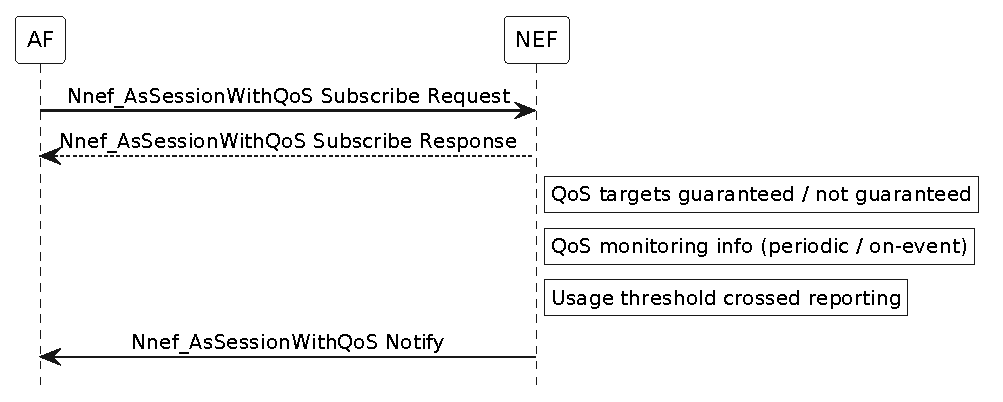
\includegraphics[width=1\linewidth]{figs/plantuml/as-session-with-qos-proposal-flow.pdf}
    \caption{Information flow for the \textit{AsSessionwithQoS} \acs{API}}
    \label{fig:flow:AsSessionWithQoSAPI}
\end{figure}

Figure \ref{fig:flow:AsSessionWithQoSAPI} highlights the described information flow for the \textit{AsSessionWithQoS} \acs{API}, obtained from the overall information flow described in TS 23.502~\cite{3GPP-23.502} and scoped to the interactions between the \acs{AF} and the \acs{NEF}, omitting internal network procedures beyond the \acs{NEF} (e.g. with the \acs{PCF}). Through this procedure, the \acs{NEF} \textit{AsSessionWithQoS} \acs{API} represents the primary programmable point in the testbed, enabling network applications to express and enforce \acs{QoS} requirements and the network conditions required to support the specific demands of each network application use case.


\subsubsection{AnalyticsExposure \acs{API}}
\label{chap:proposal:exposure:nef:AnalyticsExposure}

The \textit{AnalyticsExposure} \acs{API}, defined in \acs{3GPP} TS~29.522~\cite{ETSI_TS_129_522_V18_11_0}, allows an \acs{AF} to obtain analytics information about the network. Analytics can be retrieved through one-time fetch requests or through subscriptions, in which the \acs{NEF} notifies the \acs{AF} periodically or when specific conditions are met. Within the testbed, this \acs{API} would be the northbound interface through which the network metrics described in Section~\ref{chap:proposal:observability}, are made available to network applications.

In the \acs{5G} System, network analytics are natively produced by the \acs{NWDAF}~\cite{ETSI_TS_123_288_V18_11_0}. This function collects data scattered across multiple network functions, such as the \acs{AMF}, \acs{SMF} and \acs{UPF}, and derives new analytics from it, in the form of statistics or predictions. The \acs{NEF} then exposes these analytics to external consumers through the \textit{AnalyticsExposure} \acs{API}. However, although the specification defines the \acs{NWDAF} as the source from which the \acs{NEF} obtains analytics~\citep{ETSI_TS_123_288_V18_11_0, ETSI_TS_129_522_V18_11_0}, the \acs{AF} interacts exclusively with the \acs{NEF} and its standardized data model, making the origin of the analytics transparent to the application. The \acs{NEF} could therefore expose analytics obtained through alternative means, such as the analysis of raw \acs{IP} traffic, as long as they follow the standardized data model. This is particularly relevant for the testbed, as it would allow network application requirements and behavior to be validated without depending on an \acs{NWDAF}.

The specification defines a set of analytics events, each associated with its own analytics payload, as listed in Table~\ref{tab:proposal:exposure:nef:analytics_events}. For instance, \texttt{DN\allowbreak\_PERFORMANCE} reports the data rate, packet delay and packet loss between \acsp{UE} and an application server, while \texttt{UE\allowbreak\_COMM} characterizes the communication of \acsp{UE} with a given application, including the exchanged traffic volume.

\begin{table}[htbp]
    \centering
    \renewcommand\tabularxcolumn[1]{m{#1}}
    \begin{tabularx}{\textwidth}{|
        >{\RaggedRight\arraybackslash}m{\widthof{\texttt{NETWORK\_PERFORMANCE}}}|
        >{\RaggedRight\arraybackslash}X|}
        \hline
        \textbf{Analytics Event} & \textbf{Description} \\
        \hline
        \texttt{UE\_MOBILITY} & Location and mobility patterns of \acsp{UE}, such as tracking areas, cells or geographical coordinates where \acsp{UE} stay over time and their direction \\
        \hline
        \texttt{UE\_COMM} & Communication patterns of \acsp{UE}, such as periodicity, duration and uplink/downlink traffic volume \\
        \hline
        \texttt{ABNORMAL\allowbreak\_BEHAVIOR} & Identifies a group of \acsp{UE} or a specific \acs{UE} with abnormal behavior, e.g. being misused or hijacked \\
        \hline
        \texttt{CONGESTION} & User data congestion in a given area, or in the area where a given \acs{UE} is located \\
        \hline
        \texttt{NETWORK\allowbreak\_PERFORMANCE} & \acs{gNB} status and resource usage, communication and mobility performance, and number of \acsp{UE} in an area of interest \\
        \hline
        \texttt{QOS\allowbreak\_SUSTAINABILITY} & Statistics on past \acs{QoS} changes or likelihood of future \acs{QoS} changes in a given area \\
        \hline
        \texttt{DISPERSION} & Locations or network slices where \acsp{UE} disperse most of their data volume and session transactions, expressed as the percentage of activity generated at each location or slice\\
        \hline
        \texttt{DN\allowbreak\_PERFORMANCE} & User plane performance, namely the average and maximum traffic rate and packet delay, and average packet loss rate \\
        \hline
        \texttt{SERVICE\allowbreak\_EXPERIENCE} & Observed service experience of \acsp{UE} in an application or network slice, expressed through the average and/or variance of the observed service mean opinion score \\
        \hline
        \texttt{E2E\allowbreak\_DATA\allowbreak\_VOL\allowbreak\_TRANS\allowbreak\_TIME} & Time to complete the transmission of a specific data volume from the \acs{UE} to the \acs{AF}, or vice versa \\
        \hline
        \texttt{MOVEMENT\allowbreak\_BEHAVIOUR} & Analytics information (statistics or predictions) regarding e.g. the number, direction and velocity of \acsp{UE} during an analytics target period in a target area \\
        \hline
        \texttt{WLAN\allowbreak\_PERFORMANCE} & Quality and performance of the \acs{WLAN} connection of \acsp{UE} according to their location \\
        \hline
        \texttt{NS\allowbreak\_LOAD\allowbreak\_LEVEL} & Load level of a network slice or network slice instance \\
        \hline
        \texttt{RELATIVE\allowbreak\_PROXIMITY} & Relative proximity among a set of \acsp{UE} \\
        \hline
    \end{tabularx}
    \caption{Analytics events defined for the \textit{AnalyticsExposure} \acs{API}~\cite{ETSI_TS_123_288_V18_11_0, ETSI_TS_129_522_V18_11_0}}
    \label{tab:proposal:exposure:nef:analytics_events}
\end{table}

Figure~\ref{fig:flow:AnalyticsExposureAPI} depicts the information flow for both interaction models of the \textit{AnalyticsExposure} \acs{API}, scoped to the interactions between the \acs{AF} and the \acs{NEF}~\cite{ETSI_TS_123_288_V18_11_0, ETSI_TS_129_522_V18_11_0}. In the subscription model, the \acs{AF} specifies the analytics events of interest, optionally restricted to a set of target \acsp{UE} and to event-specific filters, together with the reporting information, such as the notification method, reporting period and maximum number of reports. The reporting information may also delimit the time period to which the analytics refer. While a past period yields statistics on observed conditions, a future period yields predictions, accompanied by a confidence level, provided that the analytics source (e.g. the \acs{NWDAF}) supports them. The request also carries the callback \acs{URI} to which the \acs{NEF} delivers the analytics notifications, according to the requested reporting information. In the fetch model, the \acs{AF} requests a single analytics event, characterized in the same way, and the analytics are returned directly in the response.

\begin{figure}[htpb]
    \centering
    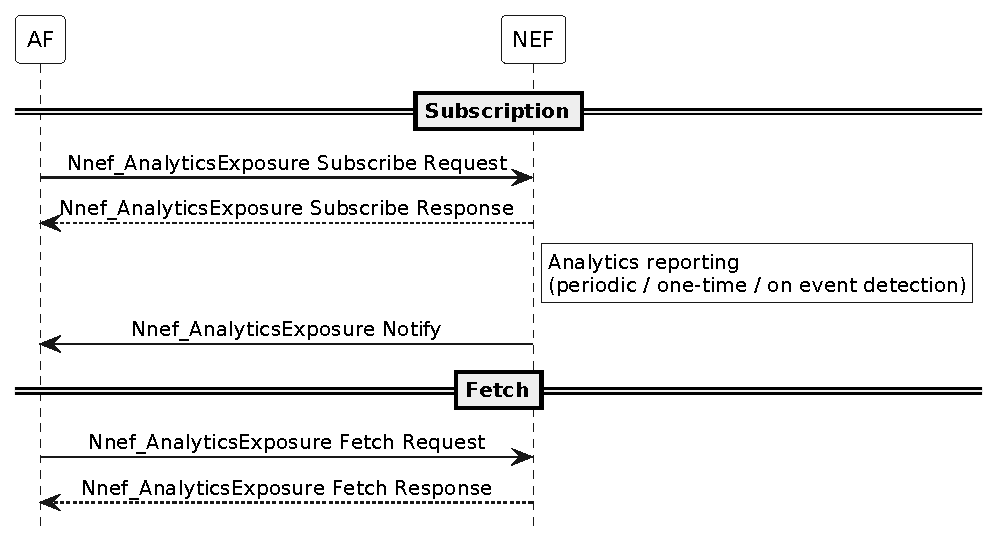
\includegraphics[width=1\linewidth]{figs/plantuml/analytics-exposure-proposal-flow.pdf}
    \caption{Information flow for the \textit{AnalyticsExposure} \acs{API}}
    \label{fig:flow:AnalyticsExposureAPI}
\end{figure}

These analytics events must be integrated with the testbed's monitoring capabilities. This way, network conditions, observed by a monitoring framework, can be exposed through the \textit{AnalyticsExposure} interface and delivered to vertical applications as they change, without the applications continuously polling the network.

In this role, the \acs{API} acts as the bridge between internal network observability and the network application layer, allowing (i) applications to adapt their behavior to the observed, and possibly future, network conditions and (ii) clients to obtain assurance that the network delivers the performance expected for their slice or \acs{QoS} session. Ultimately, the exposed analytics also support the validation of the network application's behavior against its declared requirements, discerning degraded network conditions from bad application logic.

\subsection{CAMARA \acsp{API} Integration}
\label{chap:proposal:exposure:camara}

Network application developers who wish to incorporate adaptive network behavior into their applications must interact with the network through the \acs{NEF} northbound \acsp{API} described in Section~\ref{chap:proposal:exposure:nef}. This can be accomplished in one of the following ways: (i) interacting directly with the \acs{NEF} northbound \acsp{API}, which requires familiarity with the \acs{3GPP} ecosystem, specifications and data models, imposing a significant burden on developers lacking the necessary telco expertise; or (ii) interacting with the network through CAMARA \acsp{API}, which abstract the complexity and underlying interactions with the \acs{NEF} and any other components contributing to the offered service, through a user-friendly interface.

The CAMARA initiative focuses on standardizing \acsp{API} at the northbound of the network, defining what capabilities are exposed and how application developers can interact with them to easily integrate network behavior into their applications. However, the southbound realization of those northbound \acsp{API}, i.e. their internal implementation, is deliberately left to each network operator. Nevertheless, \acs{GSMA} produces guideline documents, such as \textit{\acs{NBI} \acsp{API} Realisation in the \acs{SBI}}~\cite{gsmaNbiRealization}, describing how CAMARA \acs{API} operations can be realized through the \acsp{API} and procedures available in the operator's network, including via \acs{NEF} northbound interfaces.

The CAMARA \acsp{API} integration proposed in this section is derived from this reference realization model, mapping CAMARA operations to the corresponding \acs{NEF} interactions. Under this model, each CAMARA \acs{API} considered in the testbed has a counterpart among the \acs{NEF} northbound \acsp{API}, exposing a simplified view over the same network capability. However, not all CAMARA \acsp{API} map directly to \acs{NEF} interfaces, as some provide auxiliary functionality within the CAMARA ecosystem, such as the \textit{Application Profiles} \acs{API}. Table~\ref{tab:proposal:exposure:camara:nef_mapping} presents the \acs{NEF} and CAMARA \acsp{API} considered for the testbed, organized by the network capabilities they expose and accompanied by representative vertical use cases.

\begin{table}[htbp]
    \centering
    \renewcommand\tabularxcolumn[1]{m{#1}}
    \begin{tabularx}{\textwidth}{|
        >{\RaggedRight\arraybackslash}m{\widthof{\acs{QoS} control}}|
        >{\RaggedRight\arraybackslash}m{\widthof{\textit{AsSessionWithQoS}}}|
        >{\RaggedRight\arraybackslash}m{\widthof{Device Reachability Status,}}|
        >{\RaggedRight\arraybackslash}X|}
        \hline
        \textbf{Capability} & \textbf{\acs{NEF} \acs{API}} & \textbf{CAMARA \acs{API}} & \textbf{Use Cases} \\
        \hline
        \acs{QoS} control & \textit{AsSessionWithQoS} & \acs{QoD} & \acs{QoS} guarantees in \acs{PPDR}, eHealth,\newline live broadcasting \\
        \hline
        \acs{UE} event monitoring & \textit{MonitoringEvent} & Device Location,\newline Device Reachability Status,\newline Device Roaming Status & Geofencing,\newline fleet tracking,\newline detection of unreachable or roaming devices \\
        \hline
        Network analytics & \textit{AnalyticsExposure} & Application Profiles,\newline Connectivity Insights Subscriptions & Bitrate adaptation in video streaming,\newline detection of degraded network conditions \\
        \hline
    \end{tabularx}
    \caption{Correspondence between \acs{NEF} and CAMARA \acsp{API}}
    \label{tab:proposal:exposure:camara:nef_mapping}
\end{table}


Among these, the following subsections detail the proposed \acs{NBI} realization procedure for the \textit{Application Profiles} and \textit{Connectivity Insights Subscriptions} CAMARA \acsp{API}, which will be subject to implementation in the following chapter.

\subsubsection{Application Profiles \acs{API}}
\label{chap:proposal:exposure:camara:profiles}

The \textit{Application Profiles} \acs{API} enables network application developers to share essential information about their applications with the network and other CAMARA \acsp{API}, informing their behavior and decisions~\cite{CAMARAApplicationProfiles}. The \acs{API} focuses on defining network quality thresholds and compute resource requirements needed by the application, which naturally translate into a broad range of use cases. Across media streaming, online gaming, and video conferencing, services can benefit from the use of such an \acs{API} to verify network conditions (e.g. bandwidth, latency, jitter, packet loss) against the desired requirements and dynamically adapt their behavior accordingly. The same profile may also assist network operators in allocating resources and defining \acsp{SLA}, based on the application’s defined needs.

Figure~\ref{fig:flow:CAMARAapplicationProfiles} illustrates the \acs{NBI} realization for the \textit{Application Profiles} \acs{API}, as defined in the \acs{GSMA} reference model~\cite{gsmaNbiRealization}. Under this model, the CAMARA \acsp{API} are exposed by an Operator Platform, acting as an \acs{AF} encapsulating the \acs{NEF}, which internally defines a series of functional blocks, such as the \acs{NBI} \acs{API} Gateway, i.e. the CAMARA northbound endpoints. The Operator Platform also defines the Application Profile Storage Function, which can be considered as a stateful component (database) for storing created application profiles.

The \acs{API} exposes all the endpoints necessary to perform all \acs{CRUD} operations on an Application Profile~\cite{CAMARAApplicationProfilesRelease}. An Application Profile, expressed by the \texttt{ApplicationProfile} schema, defines application thresholds provided for network quality, including packet delay budget, minimum downstream and 
upstream rates, packet error loss rate and jitter, as well as compute resource requirements, such as target min \acs{CPU}, memory and \acs{GPU} specification.

\begin{figure}[htpb]
    \centering
    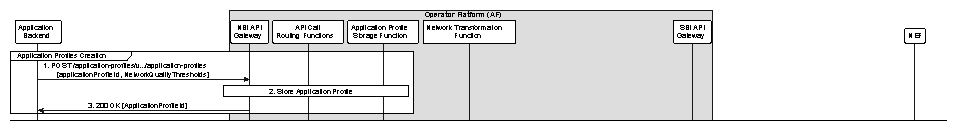
\includegraphics[width=1\linewidth]{figs/gsma-application-profiles.pdf}
    \caption{\acs{NBI} Realization for Application Profiles \acs{API}~\cite{gsmaNbiRealization}}
    \label{fig:flow:CAMARAapplicationProfiles}
\end{figure}

The sequence diagram focuses on the application profiles creation procedure. The application backend, e.g. a network application, submits a POST request to the CAMARA \acs{API} endpoint specifying the profile application requirements through the \texttt{Application\allowbreak Profile\allowbreak Request} record~\cite{CAMARAApplicationProfilesRelease}. On success, CAMARA stores the profile on the local storage repository and returns the created resource identified by a unique profile identifier. This identifier will subsequently be referenced/used in all further \acs{API} operations (retrieval, update and deletion), or by any other CAMARA \acsp{API} that consume the profile.

Throughout this workflow, there is no interaction with the \acs{NEF} or the \acs{5GC}, showcased by the absence of requests to the Network Transformation Function (i.e. the CAMARA translation layer) and the \acs{SBI} \acs{API} Gateway. This emphasizes the role of the \textit{Application Profiles} \acs{API} as a management interface over a shared profile repository, storing requirement declarations that other CAMARA \acsp{API} and network systems may reference/use to make their own decisions, as is the case of the \textit{Connectivity Insights Subscriptions} \acs{API}, discussed in the following section.

\subsubsection{Connectivity Insights Subscriptions \acs{API}}
\label{chap:proposal:exposure:camara:insights}

The \textit{Connectivity Insights Subscriptions} \acs{API} allows developers to receive continuous updates about network quality through event notifications~\cite{CAMARAConnectivityInsightsSubscriptions}. More specifically, applications can leverage this \acs{API} to monitor network conditions in real-time, receiving alerts when quality metrics fall outside the thresholds defined in their application profile, declared via the CAMARA \textit{Application Profiles} \acs{API}. Therefore, this \acs{API} represents the actual mechanism that makes the use cases specified in the previous section possible. Services which previously used profiles to declare their throughput thresholds, can now subscribe to receive notifications the moment those thresholds are breached, allowing them to take adaptive/proactive measures and prevent service disruption.

Figure~\ref{fig:flow:CAMARAconnectivityInsightsSubscriptions} illustrates the \acs{NBI} realization for the \textit{Connectivity Insights Subscriptions} \acs{API} from the \acs{GSMA} document~\cite{gsmaNbiRealization}. The procedure assumes that an application profile is previously created, as described in Section~\ref{chap:proposal:exposure:camara:profiles} (steps 1 to 3). The application then requests the creation of the analytics subscription, specifying the target device and the application server between which monitoring takes place, along with the callback endpoint (\texttt{sink}) and the referenced application profile. The application profile thus defines the network requirements to be monitored. This establishes a direct dependency between the \textit{Connectivity Insights Subscriptions} \acs{API} and the \textit{Application Profiles} \acs{API}, as a subscription requires a previously created application profile to define the criteria against which observed network conditions are evaluated.

\begin{figure}[htpb]
    \centering
    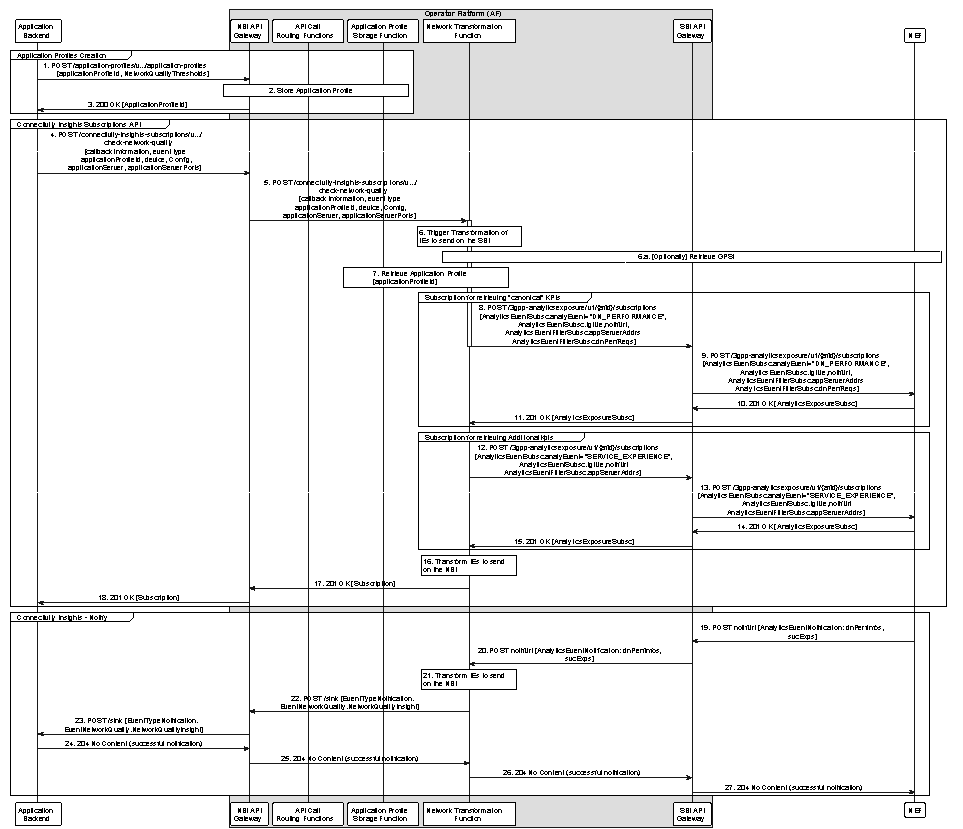
\includegraphics[width=1\linewidth]{figs/gsma-connectivity-insights-subscriptions.pdf}
    \caption{\acs{NBI} Realization for Connectivity Insights Subscriptions \acs{API}~\cite{gsmaNbiRealization}}
    \label{fig:flow:CAMARAconnectivityInsightsSubscriptions}
\end{figure}

Unlike the \textit{Application Profiles} \acs{API}, which involves no interaction with the \acs{NEF} and, consequently, no translation between the CAMARA data models and the underlying \acs{NEF} \acs{3GPP} procedures, the \textit{Connectivity Insights Subscriptions} \acs{API} encapsulates the \acs{NEF} \textit{AnalyticsExposure}~\acs{API}. After receiving the request, the CAMARA layer fetches the application profile from the datastore. The request and the retrieved profile (step 7) are then translated into one or multiple \textit{AnalyticsExposure} subscriptions, which are sent to the \acs{NEF}. The fields of the request are converted into the subscription, passing the device as the target \acs{UE} (\texttt{tgtUe}) and the addressed application server. When the device is identified by its \acs{IP} address, its \acs{GPSI} may first be retrieved from the network (step 6.a). The notification destination of each subscription (\texttt{notifUri}) is also set to the \acs{URI} of the CAMARA service, so that \acs{NEF} notifications are received by the translation layer, before being forwarded to the client. In addition, the network quality thresholds of the application profile are mapped into the reporting thresholds of the \texttt{dnPerfReqs} attribute (for the \texttt{DN\_PERFORMANCE} event), so that the \acs{NEF} notifies the Operator Platform whenever the observed performance crosses them. The reporting requirements of the subscription are, in turn, mapped into the \texttt{analyRepInfo} attribute.

The \acs{NEF} \textit{AnalyticsExposure} \acs{API} supports a wide range of analytics events, covering aspects such as network performance, \acs{UE} communication patterns and service experience~\cite{ETSI_TS_129_522_V18_11_0}. Among these, the \acs{GSMA} reference document selects two events to fulfill the analytics requirements of the \textit{Connectivity Insights Subscriptions} \acs{API}. The \texttt{DN\allowbreak\_PERFORMANCE} event is recommended to retrieve the canonical \acsp{KPI} of the application profile, i.e. the packet delay budget, the downstream and upstream rates, the packet error loss rate and the jitter. A complementary subscription for the \texttt{SERVICE\allowbreak\_EXPERIENCE} event may additionally be created to retrieve additional \acsp{KPI}, namely an indication of the radio conditions and access technology of the device, without any threshold attached.

Once the \textit{AnalyticsExposure} subscriptions are created, the reference to the CAMARA subscription is returned to the application backend. From this point forward, the communication between the involved entities, i.e. application, CAMARA and \acs{NEF}, is entirely based on callbacks. When the notification criteria are met, the \acs{NEF} sends a notification to the \texttt{notifUri} carrying the reported analytics. The CAMARA service then processes these analytics into a network quality insight, indicating, for each threshold of the application profile, if the network meets or is unable the application requirements. At the end, a second callback delivers this insight to the original \texttt{sink} specified by the application in the CAMARA subscription request.

Combined, the \textit{Application Profiles} and \textit{Connectivity Insights Subscriptions} \acsp{API} would allow a network application to declare its network requirements once and be notified whenever the network fails to meet them. The selection of analytics events, the translation into \acs{3GPP} data models and the evaluation of the reported metrics would  be completely abstracted from the consumer, allowing developers without telco expertise to incorporate network analytics into their applications.

\subsection{Secure \acs{API} Exposure via \acs{CAPIF}}
\label{chap:proposal:exposure:capif}

The \acs{NEF} and CAMARA components described in the preceding sections provide the mechanisms necessary to expose network capabilities to third parties. Together, they provide developers with the interfaces required to interact with the underlying \acs{5G} infrastructure, leveraging it to build network applications. Nevertheless, a standardized mechanism for the secure discovery, exposure, and consumption of these northbound \acsp{API} is yet to be defined.

As introduced at the beginning of this section, these northbound \acsp{API} should be exposed through a common governance mechanism, i.e. \acs{CAPIF}~\cite{ETSI_CAPIF_TS_123_222_V18_4_0}. It introduces a set of roles, namely the \acs{API} Provider, \acs{API} Invoker and \acf{CCF}, along with the procedures for \acs{API} publishing, discovery, and access control. Given its generic design, several works in the research community have treated \acs{CAPIF} as a general-purpose \acs{API} gateway with authentication and authorization capabilities, leveraging it to protect both \acs{NEF} and CAMARA northbound \acsp{API}~\citep{PathwayNaaSCAMARA,pushingBoundariesScalable5GCN}.

This dissertation follows the same interpretation, using \acs{CAPIF} as a unified secure exposure layer that consolidates common supporting capabilities into a single component, for all northbound \acsp{API} in the testbed. Under this model, (i) \acs{CCF} acts as the central control entity of the framework; (ii) both the \acs{NEF} and CAMARA \acsp{API} act as \acs{API} providers exposing interfaces to be consumed by network applications, which operate as external \acs{API} invokers; and (iii) each CAMARA \acs{API} additionally assumes the role of an internal \acs{API} invoker, interacting with \acs{NEF}'s \acs{API} to deliver its services from inside the network's trust domain.

{\spaceskip=\fontdimen2\font plus 0.5em minus \fontdimen4\font
The procedures defined in the \acs{CAPIF} architecture are realized as a collection of RESTful \acsp{API} in \acs{3GPP} TS 29.222~\cite{ETSI_CAPIF_TS_129_222_V18_6_0}, namely the \texttt{Discover\allowbreak\_Service}, \texttt{Publish\allowbreak\_Service}, \texttt{Events}, \texttt{API\allowbreak\_Invoker\allowbreak\_Management}, \texttt{Security}, \texttt{Monitoring}, \texttt{Logging\allowbreak\_API\allowbreak\_Invocation}, \texttt{Auditing}, \texttt{Access\allowbreak\_Control\allowbreak\_Policy}, \texttt{API\allowbreak\_Provider\allowbreak\_Management}, and \texttt{Routing\allowbreak\_Info} \acsp{API}.}
In the testbed, the exposure of each northbound \acs{API} would follow these procedures. Before any \acs{API} becomes available, each provider should register with the \acs{CCF} and publish its service \acs{API} information through the \acs{CAPIFAPF}. Each network application would then onboard with the \acs{CCF} to obtain its security credentials, and use the discovery interface of the \acs{CCF} to identify the exposed \acsp{API}, their endpoints, and the authorization policies governing their use. Each invocation would subsequently reach the \acs{CAPIFAEF}, which authenticates the invoker, validates the authorization issued by the \acs{CCF}, and logs the invocation for auditing. Through these onboarding and authorization policies, the set of \acsp{API} available to each network application can also be restricted~\cite{ETSI_CAPIF_TS_123_222_V18_4_0}.

As a result, rather than requiring separate onboarding, discovery, and authentication procedures for each \acs{API} suite, a single \acs{CAPIF} integration point consolidates these concerns regardless of whether the underlying \acs{API} is a \acs{3GPP} \acs{NEF} interface or a CAMARA abstraction. This significantly reduces integration complexity and aligns with the testbed's objective of providing a developer-friendly environment for the rapid development and validation of network applications.

